% Options for packages loaded elsewhere
\PassOptionsToPackage{unicode}{hyperref}
\PassOptionsToPackage{hyphens}{url}
\PassOptionsToPackage{dvipsnames,svgnames,x11names}{xcolor}
%
\documentclass[
  letterpaper,
  DIV=11,
  numbers=noendperiod]{scrartcl}

\usepackage{amsmath,amssymb}
\usepackage{iftex}
\ifPDFTeX
  \usepackage[T1]{fontenc}
  \usepackage[utf8]{inputenc}
  \usepackage{textcomp} % provide euro and other symbols
\else % if luatex or xetex
  \usepackage{unicode-math}
  \defaultfontfeatures{Scale=MatchLowercase}
  \defaultfontfeatures[\rmfamily]{Ligatures=TeX,Scale=1}
\fi
\usepackage{lmodern}
\ifPDFTeX\else  
    % xetex/luatex font selection
\fi
% Use upquote if available, for straight quotes in verbatim environments
\IfFileExists{upquote.sty}{\usepackage{upquote}}{}
\IfFileExists{microtype.sty}{% use microtype if available
  \usepackage[]{microtype}
  \UseMicrotypeSet[protrusion]{basicmath} % disable protrusion for tt fonts
}{}
\makeatletter
\@ifundefined{KOMAClassName}{% if non-KOMA class
  \IfFileExists{parskip.sty}{%
    \usepackage{parskip}
  }{% else
    \setlength{\parindent}{0pt}
    \setlength{\parskip}{6pt plus 2pt minus 1pt}}
}{% if KOMA class
  \KOMAoptions{parskip=half}}
\makeatother
\usepackage{xcolor}
\usepackage[top=1in,left=1in,right=1in,bottom=1in]{geometry}
\setlength{\emergencystretch}{3em} % prevent overfull lines
\setcounter{secnumdepth}{-\maxdimen} % remove section numbering
% Make \paragraph and \subparagraph free-standing
\makeatletter
\ifx\paragraph\undefined\else
  \let\oldparagraph\paragraph
  \renewcommand{\paragraph}{
    \@ifstar
      \xxxParagraphStar
      \xxxParagraphNoStar
  }
  \newcommand{\xxxParagraphStar}[1]{\oldparagraph*{#1}\mbox{}}
  \newcommand{\xxxParagraphNoStar}[1]{\oldparagraph{#1}\mbox{}}
\fi
\ifx\subparagraph\undefined\else
  \let\oldsubparagraph\subparagraph
  \renewcommand{\subparagraph}{
    \@ifstar
      \xxxSubParagraphStar
      \xxxSubParagraphNoStar
  }
  \newcommand{\xxxSubParagraphStar}[1]{\oldsubparagraph*{#1}\mbox{}}
  \newcommand{\xxxSubParagraphNoStar}[1]{\oldsubparagraph{#1}\mbox{}}
\fi
\makeatother

\usepackage{color}
\usepackage{fancyvrb}
\newcommand{\VerbBar}{|}
\newcommand{\VERB}{\Verb[commandchars=\\\{\}]}
\DefineVerbatimEnvironment{Highlighting}{Verbatim}{commandchars=\\\{\}}
% Add ',fontsize=\small' for more characters per line
\usepackage{framed}
\definecolor{shadecolor}{RGB}{241,243,245}
\newenvironment{Shaded}{\begin{snugshade}}{\end{snugshade}}
\newcommand{\AlertTok}[1]{\textcolor[rgb]{0.68,0.00,0.00}{#1}}
\newcommand{\AnnotationTok}[1]{\textcolor[rgb]{0.37,0.37,0.37}{#1}}
\newcommand{\AttributeTok}[1]{\textcolor[rgb]{0.40,0.45,0.13}{#1}}
\newcommand{\BaseNTok}[1]{\textcolor[rgb]{0.68,0.00,0.00}{#1}}
\newcommand{\BuiltInTok}[1]{\textcolor[rgb]{0.00,0.23,0.31}{#1}}
\newcommand{\CharTok}[1]{\textcolor[rgb]{0.13,0.47,0.30}{#1}}
\newcommand{\CommentTok}[1]{\textcolor[rgb]{0.37,0.37,0.37}{#1}}
\newcommand{\CommentVarTok}[1]{\textcolor[rgb]{0.37,0.37,0.37}{\textit{#1}}}
\newcommand{\ConstantTok}[1]{\textcolor[rgb]{0.56,0.35,0.01}{#1}}
\newcommand{\ControlFlowTok}[1]{\textcolor[rgb]{0.00,0.23,0.31}{\textbf{#1}}}
\newcommand{\DataTypeTok}[1]{\textcolor[rgb]{0.68,0.00,0.00}{#1}}
\newcommand{\DecValTok}[1]{\textcolor[rgb]{0.68,0.00,0.00}{#1}}
\newcommand{\DocumentationTok}[1]{\textcolor[rgb]{0.37,0.37,0.37}{\textit{#1}}}
\newcommand{\ErrorTok}[1]{\textcolor[rgb]{0.68,0.00,0.00}{#1}}
\newcommand{\ExtensionTok}[1]{\textcolor[rgb]{0.00,0.23,0.31}{#1}}
\newcommand{\FloatTok}[1]{\textcolor[rgb]{0.68,0.00,0.00}{#1}}
\newcommand{\FunctionTok}[1]{\textcolor[rgb]{0.28,0.35,0.67}{#1}}
\newcommand{\ImportTok}[1]{\textcolor[rgb]{0.00,0.46,0.62}{#1}}
\newcommand{\InformationTok}[1]{\textcolor[rgb]{0.37,0.37,0.37}{#1}}
\newcommand{\KeywordTok}[1]{\textcolor[rgb]{0.00,0.23,0.31}{\textbf{#1}}}
\newcommand{\NormalTok}[1]{\textcolor[rgb]{0.00,0.23,0.31}{#1}}
\newcommand{\OperatorTok}[1]{\textcolor[rgb]{0.37,0.37,0.37}{#1}}
\newcommand{\OtherTok}[1]{\textcolor[rgb]{0.00,0.23,0.31}{#1}}
\newcommand{\PreprocessorTok}[1]{\textcolor[rgb]{0.68,0.00,0.00}{#1}}
\newcommand{\RegionMarkerTok}[1]{\textcolor[rgb]{0.00,0.23,0.31}{#1}}
\newcommand{\SpecialCharTok}[1]{\textcolor[rgb]{0.37,0.37,0.37}{#1}}
\newcommand{\SpecialStringTok}[1]{\textcolor[rgb]{0.13,0.47,0.30}{#1}}
\newcommand{\StringTok}[1]{\textcolor[rgb]{0.13,0.47,0.30}{#1}}
\newcommand{\VariableTok}[1]{\textcolor[rgb]{0.07,0.07,0.07}{#1}}
\newcommand{\VerbatimStringTok}[1]{\textcolor[rgb]{0.13,0.47,0.30}{#1}}
\newcommand{\WarningTok}[1]{\textcolor[rgb]{0.37,0.37,0.37}{\textit{#1}}}

\providecommand{\tightlist}{%
  \setlength{\itemsep}{0pt}\setlength{\parskip}{0pt}}\usepackage{longtable,booktabs,array}
\usepackage{calc} % for calculating minipage widths
% Correct order of tables after \paragraph or \subparagraph
\usepackage{etoolbox}
\makeatletter
\patchcmd\longtable{\par}{\if@noskipsec\mbox{}\fi\par}{}{}
\makeatother
% Allow footnotes in longtable head/foot
\IfFileExists{footnotehyper.sty}{\usepackage{footnotehyper}}{\usepackage{footnote}}
\makesavenoteenv{longtable}
\usepackage{graphicx}
\makeatletter
\def\maxwidth{\ifdim\Gin@nat@width>\linewidth\linewidth\else\Gin@nat@width\fi}
\def\maxheight{\ifdim\Gin@nat@height>\textheight\textheight\else\Gin@nat@height\fi}
\makeatother
% Scale images if necessary, so that they will not overflow the page
% margins by default, and it is still possible to overwrite the defaults
% using explicit options in \includegraphics[width, height, ...]{}
\setkeys{Gin}{width=\maxwidth,height=\maxheight,keepaspectratio}
% Set default figure placement to htbp
\makeatletter
\def\fps@figure{htbp}
\makeatother

\usepackage{booktabs}
\usepackage{longtable}
\usepackage{array}
\usepackage{multirow}
\usepackage{wrapfig}
\usepackage{float}
\usepackage{colortbl}
\usepackage{pdflscape}
\usepackage{tabu}
\usepackage{threeparttable}
\usepackage{threeparttablex}
\usepackage[normalem]{ulem}
\usepackage{makecell}
\usepackage{xcolor}
\KOMAoption{captions}{tableheading,figureheading}
\makeatletter
\@ifpackageloaded{caption}{}{\usepackage{caption}}
\AtBeginDocument{%
\ifdefined\contentsname
  \renewcommand*\contentsname{Table of contents}
\else
  \newcommand\contentsname{Table of contents}
\fi
\ifdefined\listfigurename
  \renewcommand*\listfigurename{List of Figures}
\else
  \newcommand\listfigurename{List of Figures}
\fi
\ifdefined\listtablename
  \renewcommand*\listtablename{List of Tables}
\else
  \newcommand\listtablename{List of Tables}
\fi
\ifdefined\figurename
  \renewcommand*\figurename{Figure}
\else
  \newcommand\figurename{Figure}
\fi
\ifdefined\tablename
  \renewcommand*\tablename{Table}
\else
  \newcommand\tablename{Table}
\fi
}
\@ifpackageloaded{float}{}{\usepackage{float}}
\floatstyle{ruled}
\@ifundefined{c@chapter}{\newfloat{codelisting}{h}{lop}}{\newfloat{codelisting}{h}{lop}[chapter]}
\floatname{codelisting}{Listing}
\newcommand*\listoflistings{\listof{codelisting}{List of Listings}}
\makeatother
\makeatletter
\makeatother
\makeatletter
\@ifpackageloaded{caption}{}{\usepackage{caption}}
\@ifpackageloaded{subcaption}{}{\usepackage{subcaption}}
\makeatother

\ifLuaTeX
  \usepackage{selnolig}  % disable illegal ligatures
\fi
\usepackage{bookmark}

\IfFileExists{xurl.sty}{\usepackage{xurl}}{} % add URL line breaks if available
\urlstyle{same} % disable monospaced font for URLs
\hypersetup{
  pdftitle={Air Pollution Across the Globe},
  pdfauthor={Sneha Arya, Greer Moran, and Gabrielle Smeltzer},
  colorlinks=true,
  linkcolor={blue},
  filecolor={Maroon},
  citecolor={Blue},
  urlcolor={Blue},
  pdfcreator={LaTeX via pandoc}}


\title{Air Pollution Across the Globe}
\author{Sneha Arya, Greer Moran, and Gabrielle Smeltzer}
\date{2025-04-24}

\begin{document}
\maketitle


\section{Table of Contents:}\label{table-of-contents}

\subsection{Research Question 1}\label{research-question-1}

How does pollutant air quality index values (e.g.~Carbon Dioxide, Ozone,
Nitrogen Dioxide, and Particle Matter) impact the overall air quality
index, which are most contributing to poor air quality index?

\subsection{Plan}\label{plan}

\begin{enumerate}
\def\labelenumi{\arabic{enumi}.}
\tightlist
\item
  Load/get needed packages in an R Chunk
\item
  Read csv
\item
  Use \{dplyr\} package to use rename() to replace column names
\item
  Get linear regression model using () and summary()
\item
  Go to Dr.Hatfield and ask how to clean summary() and use kableExtra
\end{enumerate}

\begin{verbatim}

Call:
lm(formula = AQI ~ CO + Ozone + NO2 + PM, data = cleanAQIdata)

Residuals:
    Min      1Q  Median      3Q     Max 
-26.664  -3.527  -1.830   0.546 167.393 

Coefficients:
             Estimate Std. Error t value Pr(>|t|)    
(Intercept) -0.603909   0.111439  -5.419 6.05e-08 ***
CO           0.017075   0.039702   0.430  0.66715    
Ozone        0.157513   0.002338  67.371  < 2e-16 ***
NO2         -0.036205   0.013496  -2.683  0.00731 ** 
PM           0.980138   0.001264 775.385  < 2e-16 ***
---
Signif. codes:  0 '***' 0.001 '**' 0.01 '*' 0.05 '.' 0.1 ' ' 1

Residual standard error: 8.94 on 23458 degrees of freedom
Multiple R-squared:  0.9746,    Adjusted R-squared:  0.9746 
F-statistic: 2.247e+05 on 4 and 23458 DF,  p-value: < 2.2e-16
\end{verbatim}

\begin{longtable}[t]{lrrrr}
\caption{Linear Regression Summary for Pollutants impact on AQI}\\
\toprule
Pollutant & Est. Slope & Std. Error & t value & p-value\\
\midrule
(Intercept) & -0.60391 & 0.11144 & -5.41918 & 0.00000\\
CO & 0.01707 & 0.03970 & 0.43007 & 0.66715\\
Ozone & 0.15751 & 0.00234 & 67.37098 & 0.00000\\
NO2 & -0.03620 & 0.01350 & -2.68260 & 0.00731\\
PM & 0.98014 & 0.00126 & 775.38517 & 0.00000\\
\bottomrule
\end{longtable}

\begin{verbatim}
    Pollutant  Est. Slope  Std. Error     t value      p-value
1 (Intercept) -0.60390878 0.111439150  -5.4191798 6.046279e-08
2          CO  0.01707452 0.039701626   0.4300711 6.671479e-01
3       Ozone  0.15751344 0.002338001  67.3709805 0.000000e+00
4         NO2 -0.03620488 0.013496207  -2.6825964 7.310429e-03
5          PM  0.98013834 0.001264066 775.3851678 0.000000e+00
\end{verbatim}

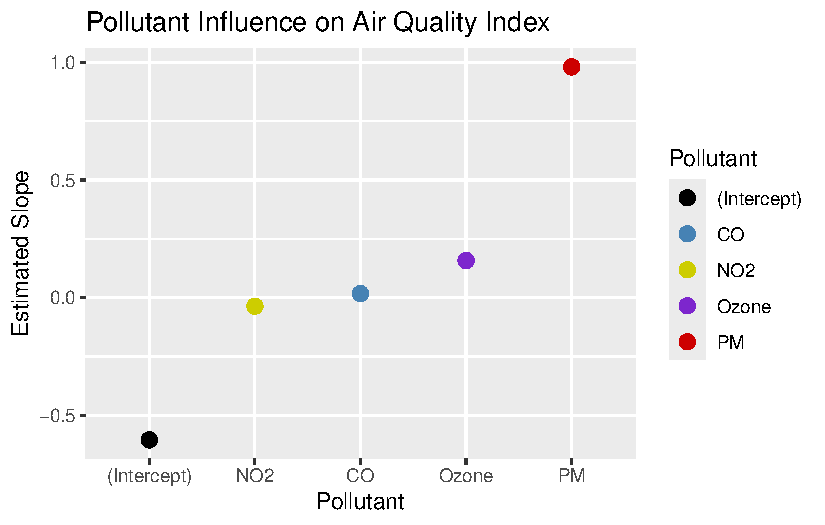
\includegraphics{FinalProject_files/figure-pdf/unnamed-chunk-2-1.pdf}

\begin{verbatim}
List of 136
 $ line                            :List of 6
  ..$ colour       : chr "black"
  ..$ linewidth    : num 0.5
  ..$ linetype     : num 1
  ..$ lineend      : chr "butt"
  ..$ arrow        : logi FALSE
  ..$ inherit.blank: logi TRUE
  ..- attr(*, "class")= chr [1:2] "element_line" "element"
 $ rect                            :List of 5
  ..$ fill         : chr "white"
  ..$ colour       : chr "black"
  ..$ linewidth    : num 0.5
  ..$ linetype     : num 1
  ..$ inherit.blank: logi TRUE
  ..- attr(*, "class")= chr [1:2] "element_rect" "element"
 $ text                            :List of 11
  ..$ family       : chr ""
  ..$ face         : chr "plain"
  ..$ colour       : chr "black"
  ..$ size         : num 11
  ..$ hjust        : num 0.5
  ..$ vjust        : num 0.5
  ..$ angle        : num 0
  ..$ lineheight   : num 0.9
  ..$ margin       : 'margin' num [1:4] 0points 0points 0points 0points
  .. ..- attr(*, "unit")= int 8
  ..$ debug        : logi FALSE
  ..$ inherit.blank: logi TRUE
  ..- attr(*, "class")= chr [1:2] "element_text" "element"
 $ title                           : NULL
 $ aspect.ratio                    : NULL
 $ axis.title                      : NULL
 $ axis.title.x                    :List of 11
  ..$ family       : NULL
  ..$ face         : NULL
  ..$ colour       : NULL
  ..$ size         : NULL
  ..$ hjust        : NULL
  ..$ vjust        : num 1
  ..$ angle        : NULL
  ..$ lineheight   : NULL
  ..$ margin       : 'margin' num [1:4] 2.75points 0points 0points 0points
  .. ..- attr(*, "unit")= int 8
  ..$ debug        : NULL
  ..$ inherit.blank: logi TRUE
  ..- attr(*, "class")= chr [1:2] "element_text" "element"
 $ axis.title.x.top                :List of 11
  ..$ family       : NULL
  ..$ face         : NULL
  ..$ colour       : NULL
  ..$ size         : NULL
  ..$ hjust        : NULL
  ..$ vjust        : num 0
  ..$ angle        : NULL
  ..$ lineheight   : NULL
  ..$ margin       : 'margin' num [1:4] 0points 0points 2.75points 0points
  .. ..- attr(*, "unit")= int 8
  ..$ debug        : NULL
  ..$ inherit.blank: logi TRUE
  ..- attr(*, "class")= chr [1:2] "element_text" "element"
 $ axis.title.x.bottom             : NULL
 $ axis.title.y                    :List of 11
  ..$ family       : NULL
  ..$ face         : NULL
  ..$ colour       : NULL
  ..$ size         : NULL
  ..$ hjust        : NULL
  ..$ vjust        : num 1
  ..$ angle        : num 90
  ..$ lineheight   : NULL
  ..$ margin       : 'margin' num [1:4] 0points 2.75points 0points 0points
  .. ..- attr(*, "unit")= int 8
  ..$ debug        : NULL
  ..$ inherit.blank: logi TRUE
  ..- attr(*, "class")= chr [1:2] "element_text" "element"
 $ axis.title.y.left               : NULL
 $ axis.title.y.right              :List of 11
  ..$ family       : NULL
  ..$ face         : NULL
  ..$ colour       : NULL
  ..$ size         : NULL
  ..$ hjust        : NULL
  ..$ vjust        : num 1
  ..$ angle        : num -90
  ..$ lineheight   : NULL
  ..$ margin       : 'margin' num [1:4] 0points 0points 0points 2.75points
  .. ..- attr(*, "unit")= int 8
  ..$ debug        : NULL
  ..$ inherit.blank: logi TRUE
  ..- attr(*, "class")= chr [1:2] "element_text" "element"
 $ axis.text                       :List of 11
  ..$ family       : NULL
  ..$ face         : NULL
  ..$ colour       : chr "grey30"
  ..$ size         : 'rel' num 0.8
  ..$ hjust        : NULL
  ..$ vjust        : NULL
  ..$ angle        : NULL
  ..$ lineheight   : NULL
  ..$ margin       : NULL
  ..$ debug        : NULL
  ..$ inherit.blank: logi TRUE
  ..- attr(*, "class")= chr [1:2] "element_text" "element"
 $ axis.text.x                     :List of 11
  ..$ family       : NULL
  ..$ face         : NULL
  ..$ colour       : NULL
  ..$ size         : NULL
  ..$ hjust        : NULL
  ..$ vjust        : num 1
  ..$ angle        : NULL
  ..$ lineheight   : NULL
  ..$ margin       : 'margin' num [1:4] 2.2points 0points 0points 0points
  .. ..- attr(*, "unit")= int 8
  ..$ debug        : NULL
  ..$ inherit.blank: logi TRUE
  ..- attr(*, "class")= chr [1:2] "element_text" "element"
 $ axis.text.x.top                 :List of 11
  ..$ family       : NULL
  ..$ face         : NULL
  ..$ colour       : NULL
  ..$ size         : NULL
  ..$ hjust        : NULL
  ..$ vjust        : num 0
  ..$ angle        : NULL
  ..$ lineheight   : NULL
  ..$ margin       : 'margin' num [1:4] 0points 0points 2.2points 0points
  .. ..- attr(*, "unit")= int 8
  ..$ debug        : NULL
  ..$ inherit.blank: logi TRUE
  ..- attr(*, "class")= chr [1:2] "element_text" "element"
 $ axis.text.x.bottom              : NULL
 $ axis.text.y                     :List of 11
  ..$ family       : NULL
  ..$ face         : NULL
  ..$ colour       : NULL
  ..$ size         : NULL
  ..$ hjust        : num 1
  ..$ vjust        : NULL
  ..$ angle        : NULL
  ..$ lineheight   : NULL
  ..$ margin       : 'margin' num [1:4] 0points 2.2points 0points 0points
  .. ..- attr(*, "unit")= int 8
  ..$ debug        : NULL
  ..$ inherit.blank: logi TRUE
  ..- attr(*, "class")= chr [1:2] "element_text" "element"
 $ axis.text.y.left                : NULL
 $ axis.text.y.right               :List of 11
  ..$ family       : NULL
  ..$ face         : NULL
  ..$ colour       : NULL
  ..$ size         : NULL
  ..$ hjust        : num 0
  ..$ vjust        : NULL
  ..$ angle        : NULL
  ..$ lineheight   : NULL
  ..$ margin       : 'margin' num [1:4] 0points 0points 0points 2.2points
  .. ..- attr(*, "unit")= int 8
  ..$ debug        : NULL
  ..$ inherit.blank: logi TRUE
  ..- attr(*, "class")= chr [1:2] "element_text" "element"
 $ axis.text.theta                 : NULL
 $ axis.text.r                     :List of 11
  ..$ family       : NULL
  ..$ face         : NULL
  ..$ colour       : NULL
  ..$ size         : NULL
  ..$ hjust        : num 0.5
  ..$ vjust        : NULL
  ..$ angle        : NULL
  ..$ lineheight   : NULL
  ..$ margin       : 'margin' num [1:4] 0points 2.2points 0points 2.2points
  .. ..- attr(*, "unit")= int 8
  ..$ debug        : NULL
  ..$ inherit.blank: logi TRUE
  ..- attr(*, "class")= chr [1:2] "element_text" "element"
 $ axis.ticks                      : list()
  ..- attr(*, "class")= chr [1:2] "element_blank" "element"
 $ axis.ticks.x                    : NULL
 $ axis.ticks.x.top                : NULL
 $ axis.ticks.x.bottom             : NULL
 $ axis.ticks.y                    : NULL
 $ axis.ticks.y.left               : NULL
 $ axis.ticks.y.right              : NULL
 $ axis.ticks.theta                : NULL
 $ axis.ticks.r                    : NULL
 $ axis.minor.ticks.x.top          : NULL
 $ axis.minor.ticks.x.bottom       : NULL
 $ axis.minor.ticks.y.left         : NULL
 $ axis.minor.ticks.y.right        : NULL
 $ axis.minor.ticks.theta          : NULL
 $ axis.minor.ticks.r              : NULL
 $ axis.ticks.length               : 'simpleUnit' num 2.75points
  ..- attr(*, "unit")= int 8
 $ axis.ticks.length.x             : NULL
 $ axis.ticks.length.x.top         : NULL
 $ axis.ticks.length.x.bottom      : NULL
 $ axis.ticks.length.y             : NULL
 $ axis.ticks.length.y.left        : NULL
 $ axis.ticks.length.y.right       : NULL
 $ axis.ticks.length.theta         : NULL
 $ axis.ticks.length.r             : NULL
 $ axis.minor.ticks.length         : 'rel' num 0.75
 $ axis.minor.ticks.length.x       : NULL
 $ axis.minor.ticks.length.x.top   : NULL
 $ axis.minor.ticks.length.x.bottom: NULL
 $ axis.minor.ticks.length.y       : NULL
 $ axis.minor.ticks.length.y.left  : NULL
 $ axis.minor.ticks.length.y.right : NULL
 $ axis.minor.ticks.length.theta   : NULL
 $ axis.minor.ticks.length.r       : NULL
 $ axis.line                       : list()
  ..- attr(*, "class")= chr [1:2] "element_blank" "element"
 $ axis.line.x                     : NULL
 $ axis.line.x.top                 : NULL
 $ axis.line.x.bottom              : NULL
 $ axis.line.y                     : NULL
 $ axis.line.y.left                : NULL
 $ axis.line.y.right               : NULL
 $ axis.line.theta                 : NULL
 $ axis.line.r                     : NULL
 $ legend.background               : list()
  ..- attr(*, "class")= chr [1:2] "element_blank" "element"
 $ legend.margin                   : 'margin' num [1:4] 5.5points 5.5points 5.5points 5.5points
  ..- attr(*, "unit")= int 8
 $ legend.spacing                  : 'simpleUnit' num 11points
  ..- attr(*, "unit")= int 8
 $ legend.spacing.x                : NULL
 $ legend.spacing.y                : NULL
 $ legend.key                      : list()
  ..- attr(*, "class")= chr [1:2] "element_blank" "element"
 $ legend.key.size                 : 'simpleUnit' num 1.2lines
  ..- attr(*, "unit")= int 3
 $ legend.key.height               : NULL
 $ legend.key.width                : NULL
 $ legend.key.spacing              : 'simpleUnit' num 5.5points
  ..- attr(*, "unit")= int 8
 $ legend.key.spacing.x            : NULL
 $ legend.key.spacing.y            : NULL
 $ legend.frame                    : NULL
 $ legend.ticks                    : NULL
 $ legend.ticks.length             : 'rel' num 0.2
 $ legend.axis.line                : NULL
 $ legend.text                     :List of 11
  ..$ family       : NULL
  ..$ face         : NULL
  ..$ colour       : NULL
  ..$ size         : 'rel' num 0.8
  ..$ hjust        : NULL
  ..$ vjust        : NULL
  ..$ angle        : NULL
  ..$ lineheight   : NULL
  ..$ margin       : NULL
  ..$ debug        : NULL
  ..$ inherit.blank: logi TRUE
  ..- attr(*, "class")= chr [1:2] "element_text" "element"
 $ legend.text.position            : NULL
 $ legend.title                    :List of 11
  ..$ family       : NULL
  ..$ face         : NULL
  ..$ colour       : NULL
  ..$ size         : NULL
  ..$ hjust        : num 0
  ..$ vjust        : NULL
  ..$ angle        : NULL
  ..$ lineheight   : NULL
  ..$ margin       : NULL
  ..$ debug        : NULL
  ..$ inherit.blank: logi TRUE
  ..- attr(*, "class")= chr [1:2] "element_text" "element"
 $ legend.title.position           : NULL
 $ legend.position                 : chr "right"
 $ legend.position.inside          : NULL
 $ legend.direction                : NULL
 $ legend.byrow                    : NULL
 $ legend.justification            : chr "center"
 $ legend.justification.top        : NULL
 $ legend.justification.bottom     : NULL
 $ legend.justification.left       : NULL
 $ legend.justification.right      : NULL
 $ legend.justification.inside     : NULL
 $ legend.location                 : NULL
 $ legend.box                      : NULL
 $ legend.box.just                 : NULL
 $ legend.box.margin               : 'margin' num [1:4] 0cm 0cm 0cm 0cm
  ..- attr(*, "unit")= int 1
 $ legend.box.background           : list()
  ..- attr(*, "class")= chr [1:2] "element_blank" "element"
 $ legend.box.spacing              : 'simpleUnit' num 11points
  ..- attr(*, "unit")= int 8
  [list output truncated]
 - attr(*, "class")= chr [1:2] "theme" "gg"
 - attr(*, "complete")= logi TRUE
 - attr(*, "validate")= logi TRUE
\end{verbatim}

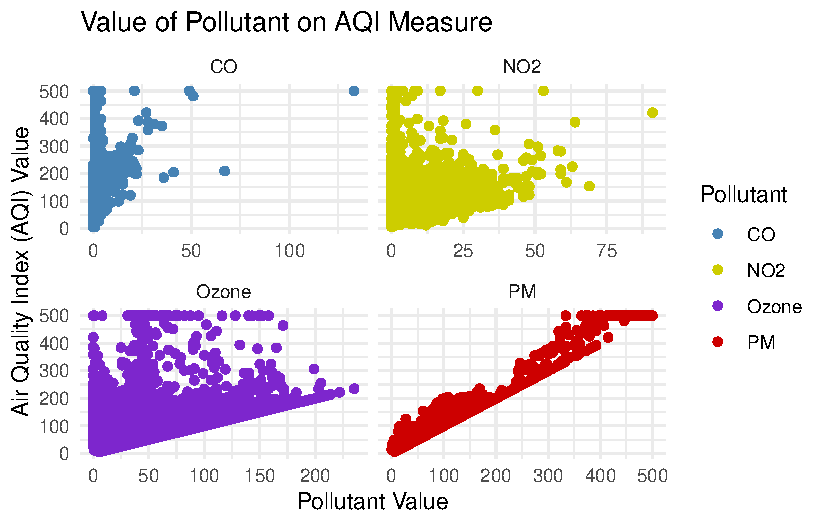
\includegraphics{FinalProject_files/figure-pdf/unnamed-chunk-2-2.pdf}

\section{An Analysis of Air Quality}\label{an-analysis-of-air-quality}

\newpage{}

\begin{figure}

\caption{\label{fig-CountryAQI}}

\centering{

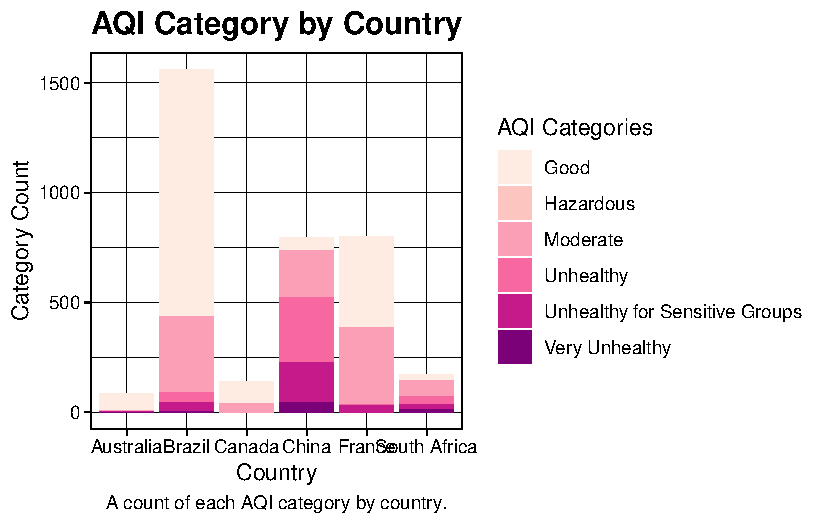
\includegraphics{FinalProject_files/figure-pdf/fig-CountryAQI-1.pdf}

}

\end{figure}%

\begin{figure}

\caption{\label{fig-UrbanpopulationAQI}}

\centering{

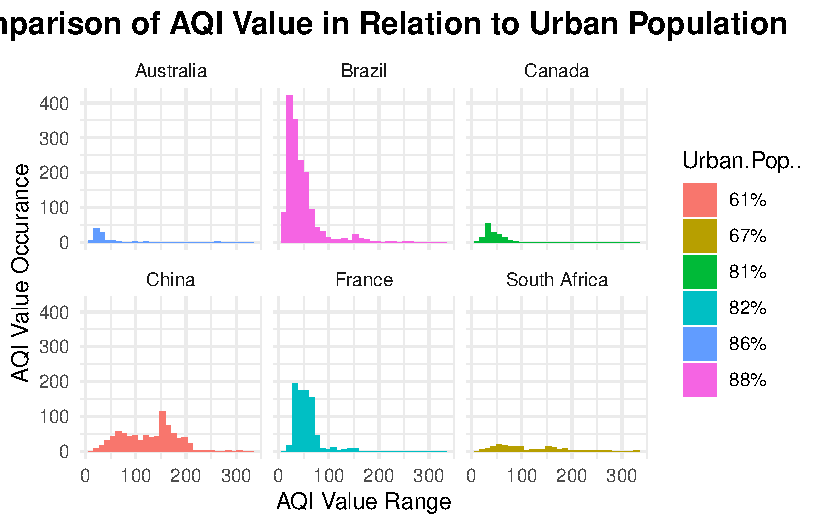
\includegraphics{FinalProject_files/figure-pdf/fig-UrbanpopulationAQI-1.pdf}

}

\end{figure}%

\begin{figure}

\caption{\label{fig-OzoneLandAreaRelation}}

\centering{

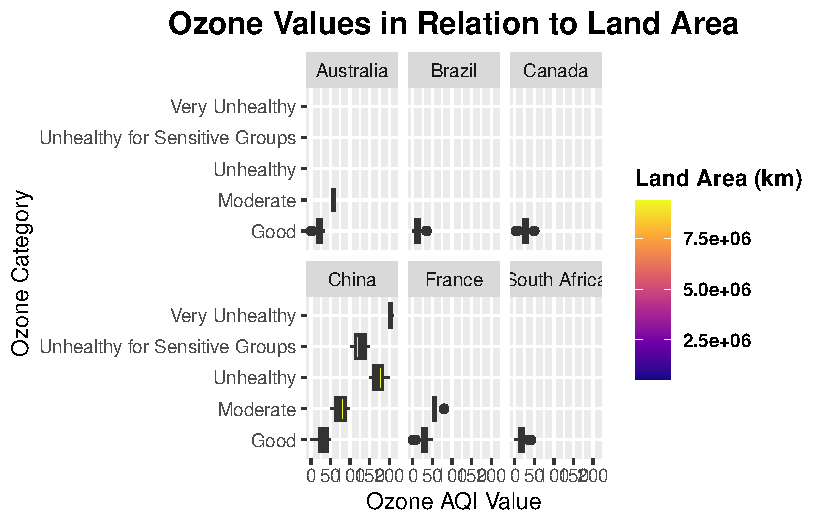
\includegraphics{FinalProject_files/figure-pdf/fig-OzoneLandAreaRelation-1.pdf}

}

\end{figure}%

\section{Data Sources and
Acknowledgement}\label{data-sources-and-acknowledgement}

\section{Code Appendix:}\label{code-appendix}

\begin{Shaded}
\begin{Highlighting}[]
\CommentTok{\# Load needed packages {-}{-}{-}}
\DocumentationTok{\#\# Must determine which are used in our code so that it is executed}


\FunctionTok{library}\NormalTok{(tidyverse)}
\FunctionTok{library}\NormalTok{(googlesheets4)}
\FunctionTok{library}\NormalTok{(knitr)}
\FunctionTok{library}\NormalTok{(dcData)}
\FunctionTok{library}\NormalTok{(tinytex)}

\CommentTok{\#| label: Data Wrangling Code for Global Air Pollution}
\CommentTok{\#| lst{-}label: Global Air Pollution, Data Wrangling}
\CommentTok{\#| lst{-}cap: "Rename Needed Columns"}


\CommentTok{\# Wrangle Air Pollution Data {-}{-}{-}}

\DocumentationTok{\#\# Get Correct Column Names {-}{-}{-}}
\DocumentationTok{\#\#\# Get Specific Data Frame of Correct Column Names}

\FunctionTok{library}\NormalTok{(dplyr)}
\FunctionTok{library}\NormalTok{(tidyverse)}
\NormalTok{globalData }\OtherTok{\textless{}{-}} \FunctionTok{read.csv}\NormalTok{(}\StringTok{"statproject.csv"}\NormalTok{)}

\NormalTok{cleanAQIdata }\OtherTok{\textless{}{-}}\NormalTok{ globalData }\SpecialCharTok{\%\textgreater{}\%}
  \FunctionTok{rename}\NormalTok{(}\FunctionTok{c}\NormalTok{(}
    \AttributeTok{AQI =} \StringTok{"AQI.Value"}\NormalTok{,}
    \AttributeTok{CO =} \StringTok{"CO.AQI.Value"}\NormalTok{,}
    \AttributeTok{Ozone =} \StringTok{"Ozone.AQI.Value"}\NormalTok{,}
    \AttributeTok{NO2 =} \StringTok{"NO2.AQI.Value"}\NormalTok{,}
    \AttributeTok{PM =} \StringTok{"PM2.5.AQI.Value"}
\NormalTok{    )}
\NormalTok{    )}

\NormalTok{aqiModel }\OtherTok{\textless{}{-}} \FunctionTok{lm}\NormalTok{(AQI }\SpecialCharTok{\textasciitilde{}}\NormalTok{ CO }\SpecialCharTok{+}\NormalTok{ Ozone }\SpecialCharTok{+}\NormalTok{ NO2 }\SpecialCharTok{+}\NormalTok{ PM, }\AttributeTok{data =}\NormalTok{ cleanAQIdata)}
\NormalTok{aqiSummary }\OtherTok{\textless{}{-}} \FunctionTok{summary}\NormalTok{(aqiModel)}
\NormalTok{aqiSummary}

\CommentTok{\# Create Table Summary Visualization {-}{-}{-}}

\NormalTok{aqiModel }\OtherTok{\textless{}{-}} \FunctionTok{as.data.frame}\NormalTok{(aqiSummary}\SpecialCharTok{$}\NormalTok{coefficients) }\DocumentationTok{\#\# create data frame}
\NormalTok{aqiModel}\SpecialCharTok{$}\NormalTok{Pollutant }\OtherTok{\textless{}{-}} \FunctionTok{rownames}\NormalTok{(aqiModel)}
\NormalTok{aqiModel }\OtherTok{\textless{}{-}}\NormalTok{ aqiModel[, }\FunctionTok{c}\NormalTok{(}\StringTok{"Pollutant"}\NormalTok{, }\StringTok{"Estimate"}\NormalTok{, }\StringTok{"Std. Error"}\NormalTok{, }\StringTok{"t value"}\NormalTok{, }\StringTok{"Pr(\textgreater{}|t|)"}\NormalTok{)]}
\FunctionTok{colnames}\NormalTok{(aqiModel) }\OtherTok{\textless{}{-}} \FunctionTok{c}\NormalTok{(}\StringTok{"Pollutant"}\NormalTok{, }\StringTok{"Est. Slope"}\NormalTok{, }\StringTok{"Std. Error"}\NormalTok{, }\StringTok{"t value"}\NormalTok{, }\StringTok{"p{-}value"}\NormalTok{)}
\FunctionTok{rownames}\NormalTok{(aqiModel) }\OtherTok{\textless{}{-}} \ConstantTok{NULL}


\FunctionTok{library}\NormalTok{(knitr)}
\FunctionTok{library}\NormalTok{(kableExtra)}
\FunctionTok{kable}\NormalTok{(}
\NormalTok{  aqiModel,}
  \AttributeTok{caption =} \StringTok{"Linear Regression Summary for Pollutants impact on AQI"}\NormalTok{,}
  \AttributeTok{digits =} \DecValTok{5}
\NormalTok{  ) }\SpecialCharTok{\%\textgreater{}\%}
  \FunctionTok{kable\_styling}\NormalTok{(}
    \AttributeTok{position =} \StringTok{"center"}
\NormalTok{  )}
\NormalTok{aqiModel}

\FunctionTok{library}\NormalTok{(ggplot2)}
\CommentTok{\# }
\FunctionTok{ggplot}\NormalTok{(}
  \AttributeTok{data =}\NormalTok{ aqiModel, }
  \AttributeTok{mapping =} \FunctionTok{aes}\NormalTok{(}
    \AttributeTok{x =} \FunctionTok{reorder}\NormalTok{(Pollutant, }\StringTok{\textasciigrave{}}\AttributeTok{Est. Slope}\StringTok{\textasciigrave{}}\NormalTok{), }
    \AttributeTok{y =} \StringTok{\textasciigrave{}}\AttributeTok{Est. Slope}\StringTok{\textasciigrave{}}\NormalTok{,}
    \AttributeTok{color =}\NormalTok{ Pollutant}
\NormalTok{    )}
\NormalTok{  ) }\SpecialCharTok{+}
  \FunctionTok{geom\_point}\NormalTok{(}
    \AttributeTok{size =} \DecValTok{3}
\NormalTok{    ) }\SpecialCharTok{+}
  \FunctionTok{labs}\NormalTok{(}
    \AttributeTok{title =} \StringTok{"Pollutant Influence on Air Quality Index"}\NormalTok{,}
    \AttributeTok{x =} \StringTok{"Pollutant"}\NormalTok{,}
    \AttributeTok{y =} \StringTok{"Estimated Slope"}
\NormalTok{  ) }\SpecialCharTok{+}
  \FunctionTok{scale\_color\_manual}\NormalTok{(}
    \AttributeTok{values =} \FunctionTok{c}\NormalTok{(}\StringTok{"black"}\NormalTok{, }\StringTok{"steelblue"}\NormalTok{, }\StringTok{"yellow3"}\NormalTok{, }\StringTok{"purple3"}\NormalTok{, }\StringTok{"red3"}\NormalTok{)}
\NormalTok{  )}
  \FunctionTok{theme\_minimal}\NormalTok{()}

\CommentTok{\# AQI Value by Pollutant Value Data Frame}
\DocumentationTok{\#\# Tidy data frame so that Pollutant is a column}
  
\NormalTok{tidyAQIdf }\OtherTok{\textless{}{-}}\NormalTok{ cleanAQIdata }\SpecialCharTok{\%\textgreater{}\%}
  \FunctionTok{pivot\_longer}\NormalTok{(}
    \AttributeTok{cols =} \FunctionTok{c}\NormalTok{(}
\NormalTok{      CO,}
\NormalTok{      Ozone,}
\NormalTok{      NO2,}
\NormalTok{      PM}
\NormalTok{    ),}
    \AttributeTok{names\_to =} \StringTok{"Pollutant"}\NormalTok{,}
    \AttributeTok{values\_to =} \StringTok{"Pollutant\_Value"}
\NormalTok{  )}

\CommentTok{\#AQI Value by Pollutant Value Scatterplots}
\DocumentationTok{\#\# Create facetted scatterplots using ggplot2}

\FunctionTok{ggplot}\NormalTok{(}
  \AttributeTok{data =}\NormalTok{ tidyAQIdf,}
  \AttributeTok{mapping =} \FunctionTok{aes}\NormalTok{(}
    \AttributeTok{x =}\NormalTok{ Pollutant\_Value,}
    \AttributeTok{y =}\NormalTok{ AQI,}
    \AttributeTok{color =}\NormalTok{ Pollutant}
\NormalTok{    )}
\NormalTok{  )}\SpecialCharTok{+}
    \FunctionTok{geom\_point}\NormalTok{() }\SpecialCharTok{+}
    \FunctionTok{facet\_wrap}\NormalTok{(}\SpecialCharTok{\textasciitilde{}}\NormalTok{ Pollutant, }\AttributeTok{scales =} \StringTok{"free\_x"}\NormalTok{) }\SpecialCharTok{+}
    \FunctionTok{labs}\NormalTok{(}
      \AttributeTok{title =} \StringTok{"Value of Pollutant on AQI Measure"}\NormalTok{,}
      \AttributeTok{x =} \StringTok{"Pollutant Value"}\NormalTok{,}
      \AttributeTok{y =} \StringTok{"Air Quality Index (AQI) Value"}
\NormalTok{    ) }\SpecialCharTok{+}
    \FunctionTok{scale\_color\_manual}\NormalTok{(}
      \AttributeTok{values =} \FunctionTok{c}\NormalTok{(}\StringTok{"steelblue"}\NormalTok{, }\StringTok{"yellow3"}\NormalTok{, }\StringTok{"purple3"}\NormalTok{, }\StringTok{"red3"}\NormalTok{)) }\SpecialCharTok{+}
    \FunctionTok{theme\_minimal}\NormalTok{()}


\FunctionTok{library}\NormalTok{(dplyr)}
\FunctionTok{library}\NormalTok{(tidyverse)}
\FunctionTok{library}\NormalTok{(ggplot2)}


\DocumentationTok{\#\# Create space for population and pollution data}
\NormalTok{pollutionData }\OtherTok{\textless{}{-}} \FunctionTok{read.csv}\NormalTok{(}\StringTok{"statproject.csv"}\NormalTok{)}
\NormalTok{populationData }\OtherTok{\textless{}{-}}\FunctionTok{read.csv}\NormalTok{(}\StringTok{"statproject1.csv"}\NormalTok{)}

\DocumentationTok{\#\# Wrangle the data for calling and combination}
\DocumentationTok{\#\# Combine the data for population}
\NormalTok{populationPollution }\OtherTok{\textless{}{-}}\FunctionTok{left\_join}\NormalTok{(}
  \AttributeTok{x =}\NormalTok{ pollutionData,}
  \AttributeTok{y =}\NormalTok{ populationData,}
  \AttributeTok{by =} \FunctionTok{join\_by}\NormalTok{(Country }\SpecialCharTok{==} \StringTok{\textquotesingle{}Country..or.dependency.\textquotesingle{}}\NormalTok{)}
\NormalTok{)}


\DocumentationTok{\#\#Filter out all cities without population}

\NormalTok{tidypopPoll }\OtherTok{\textless{}{-}}\NormalTok{ populationPollution }\SpecialCharTok{\%\textgreater{}\%}

\FunctionTok{filter}\NormalTok{(}\FunctionTok{if\_all}\NormalTok{(Population..}\FloatTok{2020.}\NormalTok{, }\SpecialCharTok{\textasciitilde{}} \SpecialCharTok{!}\FunctionTok{is.na}\NormalTok{(.)))}

\DocumentationTok{\#\#Filter our data to a country from each continent, excluding Antarctica}

\NormalTok{filteredCountry }\OtherTok{\textless{}{-}} \FunctionTok{c}\NormalTok{(}\StringTok{"Australia"}\NormalTok{, }\StringTok{"Brazil"}\NormalTok{, }\StringTok{"Canada"}\NormalTok{, }\StringTok{"China"}\NormalTok{,}\StringTok{"France"}\NormalTok{, }\StringTok{"South Africa"}\NormalTok{  )}
\NormalTok{specificCountry }\OtherTok{\textless{}{-}}\NormalTok{ tidypopPoll }\SpecialCharTok{\%\textgreater{}\%}  
  \FunctionTok{filter}\NormalTok{(Country }\SpecialCharTok{\%in\%}\NormalTok{ filteredCountry)}


\DocumentationTok{\#\#Create Comparison Visuals}

\FunctionTok{ggplot}\NormalTok{(specificCountry) }\SpecialCharTok{+}
  \FunctionTok{aes}\NormalTok{(}\AttributeTok{x =}\NormalTok{ Country, }\AttributeTok{fill =}\NormalTok{ AQI.Category) }\SpecialCharTok{+}
  \FunctionTok{geom\_bar}\NormalTok{() }\SpecialCharTok{+}
  \FunctionTok{scale\_fill\_brewer}\NormalTok{(}\AttributeTok{palette =} \StringTok{"RdPu"}\NormalTok{, }\AttributeTok{direction =} \DecValTok{1}\NormalTok{) }\SpecialCharTok{+}
  \FunctionTok{labs}\NormalTok{(}
    \AttributeTok{x =} \StringTok{"Country"}\NormalTok{,}
    \AttributeTok{y =} \StringTok{"Category Count"}\NormalTok{,}
    \AttributeTok{title =} \StringTok{"AQI Category by Country"}\NormalTok{,}
    \AttributeTok{caption =} \StringTok{"A count of each AQI category by country."}\NormalTok{,}
    \AttributeTok{fill =} \StringTok{"AQI Categories"}
\NormalTok{  ) }\SpecialCharTok{+}
  \FunctionTok{theme\_linedraw}\NormalTok{() }\SpecialCharTok{+}
  \FunctionTok{theme}\NormalTok{(}
    \AttributeTok{plot.title =} \FunctionTok{element\_text}\NormalTok{(}\AttributeTok{size =} \DecValTok{15}\NormalTok{L,}
    \AttributeTok{face =} \StringTok{"bold"}\NormalTok{,}
    \AttributeTok{hjust =} \FloatTok{0.5}\NormalTok{),}
    \AttributeTok{plot.caption =} \FunctionTok{element\_text}\NormalTok{(}\AttributeTok{hjust =} \FloatTok{0.5}\NormalTok{)}
\NormalTok{  )}
 

\NormalTok{specificCountry }\SpecialCharTok{\%\textgreater{}\%}
 \FunctionTok{filter}\NormalTok{(AQI.Value }\SpecialCharTok{\textgreater{}=} \DecValTok{10}\NormalTok{L }\SpecialCharTok{\&}\NormalTok{ AQI.Value }\SpecialCharTok{\textless{}=} \DecValTok{350}\NormalTok{L) }\SpecialCharTok{\%\textgreater{}\%}
 \FunctionTok{ggplot}\NormalTok{() }\SpecialCharTok{+}
  \FunctionTok{aes}\NormalTok{(}\AttributeTok{x =}\NormalTok{ AQI.Value, }\AttributeTok{fill =}\NormalTok{ Urban.Pop..) }\SpecialCharTok{+}
  \FunctionTok{geom\_histogram}\NormalTok{(}\AttributeTok{bins =} \DecValTok{30}\NormalTok{L) }\SpecialCharTok{+}
  \FunctionTok{scale\_fill\_hue}\NormalTok{(}\AttributeTok{direction =} \DecValTok{1}\NormalTok{) }\SpecialCharTok{+}
  \FunctionTok{labs}\NormalTok{(}
    \AttributeTok{x =} \StringTok{"AQI Value Range"}\NormalTok{,}
    \AttributeTok{y =} \StringTok{"AQI Value Occurance"}\NormalTok{,}
    \AttributeTok{title =} \StringTok{"Comparison of AQI Value in Relation to Urban Population"}
\NormalTok{  ) }\SpecialCharTok{+}
  \FunctionTok{theme\_minimal}\NormalTok{() }\SpecialCharTok{+}
  \FunctionTok{theme}\NormalTok{(}
    \AttributeTok{plot.title =} \FunctionTok{element\_text}\NormalTok{(}\AttributeTok{size =} \DecValTok{15}\NormalTok{L,}
    \AttributeTok{face =} \StringTok{"bold"}\NormalTok{,}
    \AttributeTok{hjust =} \FloatTok{0.5}\NormalTok{)}
\NormalTok{  ) }\SpecialCharTok{+}
  \FunctionTok{facet\_wrap}\NormalTok{(}\FunctionTok{vars}\NormalTok{(Country))}
\FunctionTok{ggplot}\NormalTok{(specificCountry) }\SpecialCharTok{+}
  \FunctionTok{aes}\NormalTok{(}
    \AttributeTok{x =}\NormalTok{ Ozone.AQI.Value,}
    \AttributeTok{y =}\NormalTok{ Ozone.AQI.Category,}
    \AttributeTok{fill =}\NormalTok{ Land.Area..Km..}
\NormalTok{  ) }\SpecialCharTok{+}
  \FunctionTok{geom\_boxplot}\NormalTok{() }\SpecialCharTok{+}
  \FunctionTok{scale\_fill\_viridis\_c}\NormalTok{(}\AttributeTok{option =} \StringTok{"plasma"}\NormalTok{, }\AttributeTok{direction =} \DecValTok{1}\NormalTok{) }\SpecialCharTok{+}
  \FunctionTok{labs}\NormalTok{(}
    \AttributeTok{x =} \StringTok{"Ozone AQI Value"}\NormalTok{,}
    \AttributeTok{y =} \StringTok{"Ozone Category"}\NormalTok{,}
    \AttributeTok{title =} \StringTok{"Ozone Values in Relation to Land Area"}\NormalTok{,}
    \AttributeTok{fill =} \StringTok{"Land Area (km)"}
\NormalTok{  ) }\SpecialCharTok{+}
  \FunctionTok{theme\_gray}\NormalTok{() }\SpecialCharTok{+}
  \FunctionTok{theme}\NormalTok{(}
    \AttributeTok{plot.title =} \FunctionTok{element\_text}\NormalTok{(}\AttributeTok{size =} \DecValTok{15}\NormalTok{L,}
    \AttributeTok{face =} \StringTok{"bold"}\NormalTok{,}
    \AttributeTok{hjust =} \FloatTok{0.5}\NormalTok{),}
    \AttributeTok{legend.text =} \FunctionTok{element\_text}\NormalTok{(}\AttributeTok{face =} \StringTok{"bold"}\NormalTok{),}
    \AttributeTok{legend.title =} \FunctionTok{element\_text}\NormalTok{(}\AttributeTok{face =} \StringTok{"bold"}\NormalTok{)}
\NormalTok{  ) }\SpecialCharTok{+}
  \FunctionTok{facet\_wrap}\NormalTok{(}\FunctionTok{vars}\NormalTok{(Country))}
\end{Highlighting}
\end{Shaded}





\end{document}
